The concept of overlaying a virtual architecture over a physical system is not entirely new -- in networking, for example, virtual overlay networks are routinely constructed on top of the physical infrastructure in modern systems.
On the other hand, the concept of overlaying a virtual architecture over a physical FPGA is only recently gaining traction among researchers, but is already generating a lot of excitements because of their potentials.


% \begin{center}
% \fbox{\begin{minipage}{\linewidth}
% A virtual reconfigurable architecture that overlays on top of the physical FPGA configurable fabric.
% \end{minipage}}
% \end{center}

So what is an FPGA overlay exactly?
Interestingly, because of the unique nature of FPGAs as a flexible configurable hardware, drawing up a precise definition for an FPGA overlay may not be as straightforward as it may seem. 
In this chapter, we will use the following definition as a starting point.

\begin{quote}
An FPGA overlay is a virtual reconfigurable architecture that overlays on top of the physical FPGA configurable fabric.
\end{quote}

From this definition, we can see that an FPGA overlay is a machine architecture that is able to carry out certain computation.  Furthermore, this architecture is \emph{virtual} because the overlay may not necessarily be implemented physically in the final design.  Finally, it is \emph{reconfigurable} because the overlay must be able to support customization or be reprogrammed to support more than one applications.

In other words, an FPGA overlay is a virtual layer of architecture that conceptually locates between the user application and the underlying physical FPGA similar to that shown in \figref{fig:overlay_overview}.
With this additional layer, user applications will no longer be implemented onto the physical FPGA directly.
Instead, the application will be targeted toward the overlay architecture regardless of what the physical FPGA may be.
A separate step will subsequently translate this overlay architecture, together with the application that runs on it, on to the physical FPGA.

\begin{figure}
\centering
\includegraphics[width=0.5\linewidth]{overlay_overview}
\caption{Using an overlay to form a 2-layer approach to FPGA application development.  Overlay may be designed as a virtual FPGA, or it may implement an entirely different compute architecture such as a coarse-grained reconfigurable array (CGRA), vector processor, multi-core process, or even an GPU.}
\label{fig:overlay_overview}
\end{figure}

The easiest way to understand how an FPGA overlay operates in practice, is to consider building a \emph{virtual} FPGA (\textsc{va}) using the configurable fabric of a physical FPGA (\textsc{pa}).  By doing so, you now have an FPGA overlay architecture in the form of \textsc{va} overlaying on top of \textsc{pa}.  We say that \textsc{va} is essentially ``virtual'' because architectural features of \textsc{va} such as its muxes or I/O blocks may not necessarily be present in \textsc{pa}.  Yet, if the overlay is constructed correctly, any design that was originally targeting \textsc{va} may now execute unmodified on \textsc{pa} without knowing its details.

However, the power of employing FPGA overlay is not limited to making virtual FPGAs only.
On the contrary, taking advantage of FPGA's general-purpose configurable fabric, many researchers have demonstrated the benefits of overlays that implement entirely different computing architectures such as 
multi-core processor system, coarse-grained reconfigurable arrays (CGRAs), or even general-purpose graphic processing units (GPUs).

Now, using a multi-core processor overlay as an example, it should be apparent how overlays are able to improve a software programmer's design productivity.
Instead of working with unfamiliar hardware-centric tools and design methodologies, software programmers are now possible to utilize FPGAs as accelerators simply by writing programs that target a familiar architecture.
In general, one benefit of using FPGA overlay is that it is able to bridge between the often software-inclined user and the low-level FPGA hardware fabric.

Of course, if an application can be readily accelerated on a multi-core processor overlay implemented using FPGAs, then it is understandably begging the question: why not simply run the design on an actual high-performance multi-core processor instead?
The answer to this question, indeed, is the key challenge that will guide the future research on overlay designs --- While an overlay offers many desirable features to software programmable such as improved design productivity, the additional layer on top of the physical FPGA inevitably introduces additional performance penalty to the system.
A good overlay design must therefore ensure that despite the performance penalty introduced, the overall acceleration offered by FPGA must remain competitive for the accelerator system to be worthwhile.
Furthermore, it must provided added value beyond a solution with a fixed general-purpose architecture.
One such added value is the ability to customize the overlay for the particular application or group of applications concerned for sake of performance or power-efficiency.



\iffalse

Unfortunately, and also fortunately, because of the flexibility of FPGAs, the exact definition of an overlay can sometimes be difficult to precisely define.  If you implement a Commodore 64 system on an FPGA so you can play your favorite 8-bit games on FPGA, are you implementing a game system or is it already a ``overlay'' in the form of a CPU system?
What if you now upgrade this classic system to become a massively multi-core processor system for parallel execution of game code?  Would that make it more of an overlay than the simple soft CPU core?


In the straightest sense according to the above definition, a simple soft CPU core implemented on an FPGA can be regarded as an overlay -- it is virtual as you can implement the same CPU differently on different FPGAs, providing portability and compatibility.  At the same time, it is also reconfigurable, as you can obviously execute a broad range of applications on this CPU by programming it with different software.


In practice, however, the concept of an FPGA overlay is a lot far reaching than a simple soft CPU core.  It encompasses all sorts of compute architectures one can imagine, with many of them designed specifically for the purpose of serving as an overlay.  These overlays are specifically designed for the goal at hand: for virtualization, for efficiency, for power-performance tradeoff, for design productivity, etc.  They are also specially designed for use in FPGA with low overhead.

\fi

%Sometimes such overlay may not even literally exist in the final physical design.  For example a word-based FPGA may exist only in the form of design constraint or is embedded in the design language, while its architectural features may not necessarily be implemented on the FPGA (e.g. any unused word-mux defined in the architecture doesn't need to be implemented.)  It is as opposed to constructing this word-based FPGA physically on silicon.

\subsection{Coarse-Grained Architectures}
In most cases, FPGA overlays are essentially coarse-grained architectures that are built on top of the physical fine-grained configurable fabric.
As their names suggest, the basic idea of a coarse-grained architecture is to reduce the configuration granularity of an FPGA from its physical fine-grained configurable fabric such as LUTs to one with coarser reconfiguration granularity.
In some cases, such coarse-grained blocks may refer simply to arithmetic blocks of moderate sizes such as adders, multipliers, or digital signal processing blocks of some sort.
In other cases, such coarse-grained blocks may refer to very complex microprocessors connected with sophisticated network-on-chip.
Regardless of the implementation, the central goal of any coarse-grained architecture remains the same: to improve power-performance of the system by trading off design flexibility.

%From the perspective of overlay design, coarse-grained architectures are very attractive.
%Not only do they have clearly demonstrated power-performance advantages, they are also good candidates to serve as a design productivity improvement choice.

In addition, because of their reduced configuration flexibility, coarse-grained architectures can also enable design methodologies that are more productive than traditional hardware design flow.
In particular, coarse-grained architectures improve a designer's productivity in two important ways.
First, by constraining the flexibility of an FPGA, a coarse-grained architecture reduces the design space significantly, which has a net effect of reducing implementation tool flow run time considerably \cite{lavin2011}. 
In addition, many coarse-grained architectures implement compute models that are more familiar to software designers, considerably lowering the barrier-to-entry to employ such designs.  For instance, many recent overlays are implemented as coarse-grained reconfigurable arrays (CGRAs), where computation is carried out by a connected array of processing elements (PEs).
Instead of implementing the user application using low-level configurable logic of the FPGA, these operations are translated into computational tasks that take place in the PEs.
To many software programmers, programming a parallel processor array, while a daunting task in its own right, is arguably a lot more approachable than to implement designs on the native FPGA configurable fabric.
As such, it is not surprising that many recent overlay designs are built on top of an underlying coarse-grained reconfigurable array \cite{kissler2006dynamically,ferreira2011fpga,shukla2006quku,Lin:2012:EDC:2460216.2460227,capalijia2013pipelined,dspoverlay}.





\section{Benefits of Overlays}
As a virtualization layer that sits between a user application and the physical configurable fabric, an FPGA overlay inherits many of the benefits that software programmers have learned to expect from their CPU virtualization experience --- portability, compatibility, manageability, isolation, etc.  On top of that, employing FPGA overlays has also been demonstrated as a good way to improve a designer's productivity through improved compilation speed and better debugging support.  Along the same line, by carefully partitioning the complex hardware-software design flow around an intermediate overlay layer, it is also possible to provide separation of concerns between software and hardware engineers in the design team.
The overlay essentially acts as a bridge between the two teams, while allowing the overall system to take advantage of the FPGA resources efficiently.

\subsection{Virtualization}
Virtualization of FPGA resources has long been an active area of research since the early days of reconfigurable computing.  These pioneering works have demonstrated many of the possibilities as well as challenges associated with virtualizing hardware resources that are not designed to be time-multiplexed.  A common trend among these early works was that virtualization can be used as a mean to provide the designers and/or tools the illusion of having infinite hardware resources.  Early works by Trimberger et al~\cite{Trimberger97}, virtual wire\cite{virtualwire} and SCORE \cite{score}, for instances, gave the users the illusion of a system with unlimited FPGA resources through carefully structured hardware/CAD system.  Others have studied the problem of time-sharing of FPGA resources from an operating system's perspective as a way to provide shared accelerator resources among users/processes. \cite{Lubbers:2009:RMP:1596532.1596540,SoTECS08,Fu:2005:FCCM}.

As the concept of FPGA overlay continues to mature, the idea of virtualizing FPGAs has taken on a new focus.  As an overlay, virtualizing FPGAs allows an additional benefit of providing a compatibility and portability layer for FPGA designs.  In the work of Zuma~\cite{zuma2012}, for instance, virtual, embedded FPGAs were proposed.  By providing a virtual FPGA layer, the authors demonstrated that it is possible to execute the same netlist on multiple FPGAs from competing vendors using multiple different design tools.

\iffalse
\subsection{Improved Design Productivity}
An important benefit of using FPGA overlays is that they promise to improve designer's productivity in developing FPGA applications.
Design productivity is hard to measure, but has long been regarded as one of the key barrier-to-entry for novice users to start using FPGAs for their applications \cite{SoFpl06}.
In particular, FPGA overlays are particularly helpful in addressing two important aspects of this design productivity challenges: 
\begin{itemize}
\item Reduced compilation time
\item Application debug
\end{itemize}
\fi

\subsection{Reduced Compilation Time}
A key difference in design experience between software compilation and implementing FPGA designs rests on their drastically different run time of the involved tools.
With modern compiler technologies, software compilation has already become a straightforward, predictable, and most importantly, very rapid process.
Compiling even a relatively complex piece of software application rarely take longer than a few minutes on a reasonably fast computer.
On the other hand, implementing applications for FPGAs involves a complex labyrinth of low-level tools that are convoluted, unpredictable, and takes a long time to complete.
Compiling even the smallest design may take tens of minutes, while spending hours or even days on some of the largest designs are not unheard of.
Unfortunately, this 2 orders of magnitude difference in run time, together with the unpredictable nature\footnote{Placing and routing a design on nearly full FPGA, for example, may or may not succeed depending on the random algorithms involved.} and the often-mystical error reporting mechanisms\footnote{To see this, try to explain to a first-time software programmer why a functionally correct design in simulation may end up with an error message about timing violation on a net with an unknown name in the report.  Then, also try to explain to the programmer how to resolve that timing error.}, are all contributing to a very high barrier-to-entry that shies away most first time software programmers.
Technically, this much longer run time of the tools also significantly reduces the number of possible debug-edit-implement cycles per day, causing project delays as well as lowered productivity of the designers.

By using an overlay as intermediate compilation target, together with careful crafting of the design process, researchers have demonstrated how such lengthy hardware development process can be reduced significantly.
For example, in the work of Intermediate Fabric\cite{Coole2010Intermediate}, an intermediate coarse-grained reconfigurable fabric was introduced as an overlay.
With the overlay architecture, the average place and route times for the tested benchmark were significantly reduced by more than 500 times.

Similarly in the work of QuickDough, a coarse-grained reconfigurable array was used as overlay to accelerate compute intensive loop kernels.  Loops are scheduled to execute on the CGRA instead of compiling to the reconfigurable fabric.  As a result, when compared to manually generating custom hardware for the loops using standard hardware tools, up to 3 orders of magnitude reduction in compilation time was demonstrated.

\subsection{Improved Debugging Capabilities}
Unlike many software development frameworks where a range of debugging facilities and methodologies are readily available, tools for debugging applications that target FPGA-based systems are still in their infancy.
Traditional FPGA design methodologies rely heavily on cycle-accurate simulations for application development and debugging.
While such simulations are invaluable to understand the low-level operation of the FPGA, they are slow, tedious and provide only limited information about the run-time behavior of the design.
To monitor run-time behavior of a design, users must rely on even more complex in-system emulation facilities or even external testing hardware.
Taking advantage of FPGA overlays, researchers have demonstrated some promising results addressing the need for better debugging tools.

For instance, in a series of work by Hung and Wilton \cite{Hung:2014:VLSI,Hung:2013:TSO:2435264.2435272}, an overlay network was incorporated into FPGA design to facilitate insertion of trace buffers after a design has been placed and routed.
By carefully controlling the signal routes to utilize only unoccupied resources in the FPGA, they have demonstrated efficient ways to dynamically select and monitor signals during run time.

In other cases, since the overlay layer enables a virtual computing paradigm for the application developer that is different from the underlying FPGA, they also enable new debugging strategies that are more suitable to the designer. For instance in MARC, debugging the user-specified OpenCL applications that run on the generated multi-core architecture can follow traditional software debugging methodologies instead of relying on low level FPGA tools.
Not only can it greatly increase the abstraction level, but it can also allow a debugging strategy that matches the user's expectation.

\subsection{Separation of Hardware and Software Concerns}
With careful planning, it is also possible to take advantage of the 2-layer design approach offered by FPGA overlays as a natural division point between hardware and software development efforts.
Recall from \figref{fig:overlay_overview} that implementing designs via an FPGA overlay involves 2 steps: user applications must first be mapped to the overlay architecture, which is subsequently implemented to the physical fabric in a second step.
In many cases, the overlay architectures are designed so they can efficiently support the computational model expected by the model.
As a result, mapping of software applications to the overlay is usually more intuitive to software programmers than to map the same application to the physical FPGA fabric in one step.
On the other hand, mapping the overlay and the user application to the physical fabric involves intimate knowledge about the FPGA hardware implementation process.
This task is best left to a separate hardware team.
Consequently, one benefit of having an overlay is that the hardware team may now devote their efforts exclusively on implementing the relatively well-structured overlay on the fabric, rather than to implement many individual applications.
The hardware team can be more focused, and can perceivably create a better, highly optimized hardware design.

For example in the work of MARC\cite{lavin2011}, a multi-core processor-like architecture was used as an intermediate compilation target.
In this project, user applications are expressed as OpenCL programs.
To implement these applications, they are first compiled as an application-specific multi-core processor, which is subsequently implemented on the physical FPGA in a separate process.
With this set up, users no longer need to understand the detailed implementation of their algorithm on FPGAs.
Instead, they write essentially standard OpenCL programs, and focuses exclusively on writing the best code for the accelerated architecture assumed.
The task to map their OpenCL code into custom core on the target overlay, and to implement that overlay on the FPGA fabric, was left to a separate team.

In their case studies, the resulting application achieves about one third of the speedup when compared to fully custom designs.
Yet with the 2-layer approach using OpenCL, the design effort with MARC is significantly lower when compared to making a custom design of the same application.




